\documentclass{article}
\usepackage[utf8]{inputenc}
\usepackage[english]{babel}
\usepackage{amsthm}
\usepackage{amsmath}
\usepackage{amssymb}
\usepackage{mathtools}
\usepackage{enumerate}
\usepackage{chngcntr}
\usepackage{sectsty}
\usepackage{xfrac}
\usepackage{hyperref} % Uncommment to make references clickable
\usepackage[a4paper,margin=1.5in,footskip=0.25in]{geometry}

% Configuring style of references
\hypersetup{
    colorlinks = True,
    allcolors = blue	
}

% Makes equation numbering based on section
\counterwithin{equation}{section}

% Changing the styling of section and subsection titles. Comment to get default styling
\sectionfont{\centering\mdseries\scshape}
\subsectionfont{\mdseries\scshape}

%%%%%%%%%%%%%%%%%%%%%%%%%%% Defining environments %%%%%%%%%%%%%%%%%%%%%%%%%%%%%%%%%%%%%%%%
\newtheoremstyle{slimDefinitionStyle} % name
    {\topsep}                    	  % Space above
    {\topsep}                    	  % Space below
    {}			                   	  % Body font
    {}                           	  % Indent amount
    {\mdseries\scshape}			  	  % Theorem head font
    { ---}                            % Punctuation after theorem head
    {.5em}                       	  % Space after theorem head
    {}  % Theorem head spec (can be left empty, meaning ‘normal’)
\newtheoremstyle{slimTheoremStyle} 	% name
    {\topsep}                    	% Space above
    {\topsep}                    	% Space below
    {\itshape}                   	% Body font
    {}                           	% Indent amount
    {\mdseries\scshape}			 	% Theorem head font
    { ---}                          % Punctuation after theorem head
    {.5em}                       	% Space after theorem head
    {}  % Theorem head spec (can be left empty, meaning ‘normal’)
\theoremstyle{slimTheoremStyle} % Comment this to get boldface theorem headers

\newtheorem{theorem}{Theorem}[section]
\newtheorem{corollary}{Corollary}[theorem]
\newtheorem{lemma}[theorem]{Lemma}
\newtheorem{proposition}[theorem]{Proposition}

% \theoremstyle{definition}
\theoremstyle{slimDefinitionStyle}
\newtheorem{definition}{Definition}[section]

\theoremstyle{remark}
\newtheorem{remark}{Remark}[section]
\newtheorem{notation}{Notation}[section]

%%%%%%%%%%%%%%%%%%%%%%%%%% Defining custom commands %%%%%%%%%%%%%%%%%%%%%%%%%%%%%%%%%%%%%%%
% Common fonts
\renewcommand{\cal}[1]{\mathcal{#1}}
\newcommand{\bb}[1]{\mathbb{#1}}

% Common sets
\newcommand{\R}{\mathbb{R}}
\newcommand{\N}{\mathbb{N}}
\newcommand{\Z}{\mathbb{Z}}

% Expectation
\newcommand{\E}{\mathbb{E}}
\newcommand{\Ex}[1]{\mathbb{E}\left[ #1 \right]}
\newcommand{\ExCond}[2]{\mathbb{E} \left[\left. #1 \right| #2 \right]}

% Probability
\renewcommand{\P}{\mathbb{P}}
\renewcommand{\Pr}[1]{\mathbb{P} \left( #1 \right)}
\newcommand{\PrCond}[2]{\mathbb{P} \left( \left. #1 \right| #2 \right)}

% Common distributions 
\newcommand{\dNorm}[2]{\mathcal(N)\left( #1, #2 \right)}
\newcommand{\dExp}[1]{\text{Exp} \left( #1 \right)}
\newcommand{\dBer}[1]{\text{Ber} \left( #1 \right)}
\newcommand{\dPoi}[1]{\text{Po} \left( #1 \right)}

% Miscellaneous math stuff
\newcommand{\defeq}{\vcentcolon=}
\newcommand{\eqdef}{=\vcentcolon}
\DeclarePairedDelimiter\ceil{\lceil}{\rceil}
\DeclarePairedDelimiter\floor{\lfloor}{\rfloor}

%%%%%%%%%%%%%%%%%%%%%%%%%%%%%%%%%%%%%%%%%%%%%%%%%%%%%%%%%%%%%%%%%%%%%%%%%%%%%%%%%%%%%%%%%%%


\begin{document}

\section{Introduction and construction}\label{dec:introduction}

\begin{quote}
{\small We introduce the main objects of study and briefly describe the construction of the corresponding stochastic processes. The construction gives rise to important properties that we discuss. }
\end{quote}

\subsection{Introduction}\label{ssec:introduction}
The East process is an interacting particle system evolving with a Glauber like dynamics on the state space $\Omega \defeq \{0,1\}^\Z$. It belongs to a class of stochastic processes called kinetically constrained spin models (KCMs), with the East process being the first of these to be studied rigorously. The process evolves as follows: at each site $x \in \Z$ the system tries to update the value of the spin at $x$ to 1 or 0 at rate $p \in (0,1)$ and $q \defeq 1 - p$ respectively. The update is accepted only if a local constraint is satisfied, which in the East process's case is that the occupation variable at site $x-1$ must be equal to 1. Sometimes we will call elements of $\Omega$ \textit{configurations} and say a site is \textit{occupied} or \textit{infected} if its spin value is equal to 1. \\

In the sections to follow we focus on two objects of interest related to the East process. The first one is the speed of the so-called \textit{front}. Consider an East process started from the configuration equal to all 0 except at the origin. It is easy to see that the spins on $(-\infty, 0]$ stay frozen for all time, and infection 'spreads' to the right. A natural question to ask then is how fast this spreading of infection happens \textit{if} it happens at all. We define the front to be the rightmost infected site in the configuration at time $t$. In our study of the speed of the front we will compare the East process to a second stochastic process called the one-sided contact process. The one-sided contact process has the same state space $\Omega$ and evolves as follows: each site \textit{recovers} i.e. sets its spin to 0 at rate $q$ and gets infected by its left neighbour (provided the neighbour is infected) at rate $p$. The second object of interest is the \textit{mixing time} of the East process when restricted to $\{ 0, 1, ..., L\}$ for some $L \in \N^+$. We will study the mixing time for the East process on $\{ 0, 1, ..., L\}$ with the occupation variable of the origin fixed to be $1$, so that the evolution at site 1 is unconstrained. \\

The main results of this paper can be summarised as follows. We show that for $p$ larger than a critical value the front of the East process started from exactly one infection propagates at precisely linear speed. We also show that for such $p$ the mixing time on $\{ 0, 1, ..., L\}$ is $\Theta(L)$\footnote{We say $f = \Theta(g)$ if there exist constants $K_1, K_2$ such that for all large enough $n \in \N$ it holds that $K_1 g(n) \leq f(n) \leq K_2 g(n)$.}. In the process of proving these we show exponential bounds on the front propagation and survival time of the one-sided contact process. The results concerning the East process have been known to hold under weaker restrictions on $p$ for some time, see \cite{ganguly2015cutoff} for a review. The results concerning the one-sided contact process were first stated in \cite{durrett1983supercritical}, but to our knowledge never proved in detail. The paper is broken into 5 chapters. The second chapter contains the statements of our main results. Chapter three discusses the one-sided contact process and presents proofs of the above mentioned exponential bounds. Chapter four is devoted to the proof of Theorem \ref{main_thm:speed} while in chapter five we present the proof of Theorem \ref{main_thm:mixing}. 


\subsection{Constructing the basic coupling}
Let $\scr{C} = (E_{x,k}, B_{x,k})_{x \in \Z, k \in \N^+}$ be a collection of independent random variables with $E_{x,k} \sim \dExp{1}$ and $B_{x,k} \sim \dBer{p=1-q}$. Define the times 
\[
T_{x,n} \defeq \sum\limits_{k=1}^n E_{x,k}
\]
 also referred to as \textit{clock rings} and call a clock ring $T_{x,n}$ \textit{legal} if the local constraint of the corresponding process is satisified at site $x$ at time $T_{x,n}$. We can now construct the East process $(\sigma_t)_{t \geq 0}$ and the one-sided contact process $(\eta_t)_{t \geq 0}$ using $\scr{C}$ as follows. 
 
For each site $x \in \Z$ at each time $T_{x,n}$:
\begin{itemize}
  \item If $B_{x,n} = 1$:
  \begin{enumerate}
  	\item If $\sigma_{T^-_{x,n}} (x-1) = 1$ update $\sigma$ to 1 at site $x$. 
  	\item If $\eta_{T^-_{x,n}} (x-1) = 1$ update $\eta$ to 1 at site $x$. 
  \end{enumerate}
  \item Else:
  \begin{enumerate}
  	\item If $\sigma_{T^-_{x,n}} (x-1) = 1$ update $\sigma$ to 0 at site $x$. 
  	\item Update $\eta$ to 0 at site $x$. 
  \end{enumerate}
\end{itemize}

\begin{figure}[!h]
  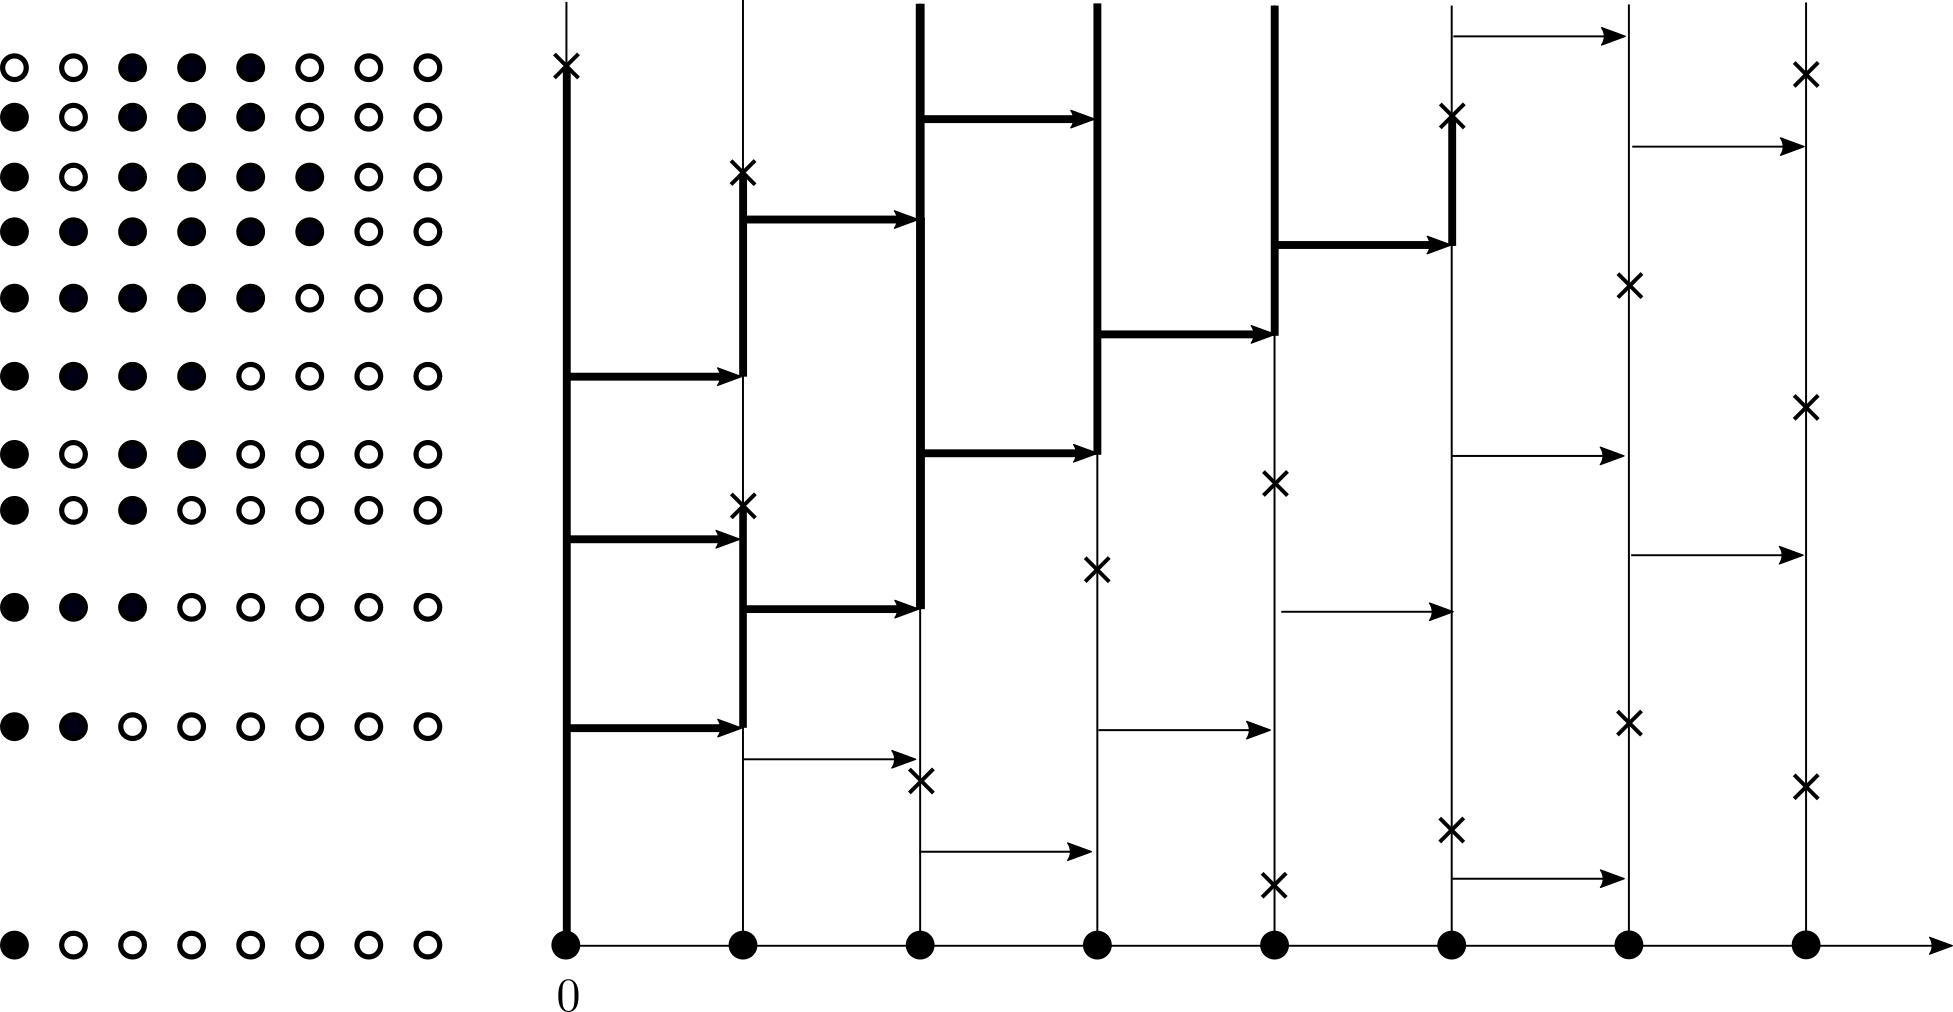
\includegraphics[width=\linewidth]{images/graphical_construction}
  \caption{Harris' graphical representation, showing the evolution of a one-sided contact process started from site $0$. }
  \label{fig:graphical_construction}
\end{figure}

There is a graphical representation of $\scr{C}$ introduced by Harris that is a helpful tool for visualizing the evolution of the two coupled processes however we will only use it to analyze the one-sided contact process. We will use the symbol $\scr{P}$ to refer to this graphical construction which we informally describe as follows. First draw vertical lines from $0$ to infinity at each integer in $\Z$. At each site $x \in \Z$ put a cross on the line at $(x, T_{x,n})$ if $B_{x,n} = 0$. If $B_{x,n} = 1$ instead of a cross draw an arrow from $(x - 1, T_{x,n})$ to $(x, T_{x,n})$. Crosses represent recovery while arrows represent infection spreading towards the right. For an example of the graphical representation see Figure \ref{fig:graphical_construction}. 

\begin{notation}[Initial configurations]
Suppose we start a stochastic process $(\xi_t)_{t \geq 0}$ with state space $\Omega$ from initial configuration $\zeta \in \Omega$. The resulting process will be denoted $(\xi^\zeta_t)_{t \geq 0}$. If $\nu$ is a probability distribution on $\Omega$, then we write $(\xi^\nu_t)_{t \geq 0}$ for the process started from a \textit{random} distribution drawn from $\nu$. The initial distribution is drawn independently from $\scr{C}$
\end{notation}
\begin{notation}[$\Omega$ and $\cal{P}(\Z)$]\label{not:powerset}
Because of the natural bijection between the power set of $\Z$ and $\Omega$, we will consider configurations as both subsets of $\Z$ and elements of $\Omega$, regularly switching between the two interpretations. 
\end{notation}

In what follows we only consider contact processes with $p > p_c$ where $p_c$ is the critical parameter for the one-sided contact process, defined as $p_c \defeq \sup\{ p : |\eta^{\{0\}}_t| \rightarrow 0\ a.s.\}$. A one-sided contact process with rates satisfying this condition is called supercritical. By definition the extinction time $\tau(\eta^{\{0\}}_.) \defeq \inf\{t \geq 0 \mid \eta^{\{0\}}_t = \varnothing \}$ of a supercritical one-sided contact process satisfies $\Pr{\tau(\eta^{\{0\}}_.) = \infty} > 0$ i.e. the process survives forever with positive probability. 

\begin{notation}[Supercritical East process]
As per the previous discussion, we call an East process supercritical if $p > p_c$. 
\end{notation}

\subsection{Domination and other properties}\label{ssec:intro_properties}
The basic coupling has two important properties that follow immediately from its definition. First, it lets us construct both processes started from any initial configuration on the same probability space. The second property is domination: if at some time $t \geq 0$ it holds that $\eta_t \leq \sigma_t$ then $\eta_{t+s} \leq \sigma_{t+s},\ \forall s \geq 0$. To see this note that under the graphical construction $\eta$ updates a particular site to 1 only if $\sigma$ does too, and $\sigma$ updates a particular site to 0 only if $\eta$ does too. In particular, if $X(\cdot)$ denotes the position of the front then $X(\eta_{t+s}) \leq X(\sigma_{t+s}),\ \forall s \geq 0$. \\

Domination is what enables us to bound the East process from below by the one-sided contact process. The reason we might want to do this is that contact processes posess desirable qualities that KCMs in general might not. Contact processes are \textit{attractive} in the sense that if $\nu \subseteq \xi \subseteq \Z$ then $\eta^\nu_t \leq \eta^\xi_t$ for all $t \geq 0$ under the basic coupling. Moreover they are also \textit{additive}: if $\nu, \xi \subseteq \Z$ then $\eta^{\nu \cup \xi}_t = \eta^\nu_t \cup \eta^\xi_t$ for all $t \geq 0$ under the basic coupling. These qualities make contact processes more amenable to analysis than KCMs, and there is a breadth of methods and results already established. The East process lacks both attractivity and additivity, thus the desire to compare it to the `simpler' one-sided contact process is justified. 


\section{Front propagation --- Proof of Theorem $2$}

\begin{quote}
{\small We prove linear speed for the front of the East model. The upper bound follows from classical results for Poisson point processes, while the lower bound is established by a comparison with the one-sided contact process, closely following the arguments of \cite{blondel2018front}. }
\end{quote}

\subsection{Restart argument}

\begin{theorem}\label{thm:restart_coupling}
For each $p < 1$ with $\frac{p}{1-p} > \lambda_c$ there exists a process $(\sigma_t, \eta_t)_{t \geq 0}$ taking values in $\Omega^2$ and a random variable $T$ taking values in $[0, \infty)$ such that 
\begin{enumerate}[(i)]
  \item $(\sigma_t)$ is a (supercritical) East model with rate parameter $p$ started from $\{0\}$
  \item $\forall t \geq 0$ and $\forall x \in \Z$, it holds that $\eta_t(x) \leq \sigma_t(x)$
  \item $(\eta_{T+t})_{t \geq 0}$ is a surviving one-sided contact process started from $\{0\}$
\end{enumerate}
Furthermore $T$ has exponentially decaying tail probabilities. 
\end{theorem}

\begin{proof}
Let $\{ \scr{C}^{(i)}\}_{i \in \N^+}$ be independent copies of $\scr{C}$. Denote by $\eta^{(i)}_.$ the one-sided contact process started from $\{0\}$, constructed using $\scr{C}^{(i)}$. Furthermore let $U_i \defeq \tau(\eta^{(i)}_.)$ be the extinction time of $\eta^{(i)}_.$. Note that the $U_i$ are i.i.d. and $\mu \defeq \Pr{U_1 = \infty} > 0$ by supercriticality. Define $L \defeq \min \{ i: U_i = \infty \}$ and note that $L$ has geometric distribution. Finally, let 
\[
T \defeq 
\left\{
  \begin{array}{ll}
    0                           & \mbox{if } L = 1 \\
    \sum\limits^{L-1}_{i=1} U_i & \mbox{otherwise}
  \end{array}
\right..
\]
First we show that $T$ has exponentially decaying tail probabilities. Note that since $T \geq 0$ almost surely, this is equivalent to finiteness of $\Ex{e^{s T}}$ for some $s > 0$. To see the latter holds for $T$ observe that conditional on $L$ the random variables $U_1, ..., U_{L-1}$ are i.i.d. with distribution equal to that of $U_1$ given $U_1 < \infty$. From Corollary \ref{cor:durrett} it follows that $U_1 | \{U_1 < \infty \}$ has exponentially decaying tail probabilities:
\begin{align*}
\Pr{U_1 > t\ | U_1 < \infty} = \frac{\Pr{t < U_1 < \infty}}{\Pr{U_1 < \infty}} \leq \frac{C e^{- \gamma t}}{1 - \mu}
\end{align*}
Therefore there exists $s > 0$ such that $\ExCond{e^{sU_1}}{U_1 < \infty} < \infty$, and so
\begin{align*}
\Ex{e^{sT}} &= \Ex{\ExCond{\exp\left(s\sum\limits_{i=1}^{L-1} U_i \right)}{L}} \\
            &= \Ex{\ExCond{e^{s U_1}}{U_1 < \infty}^{L-1}} < \infty \,,
\end{align*}
where finiteseness follows as $L$ has geometric distribution and so finite moment generating function for all $s \in \R$. \\
Now we construct the process $(\sigma_t, \eta_t)_{t \geq 0}$:
\begin{enumerate}
  \item Let $(\sigma^{[1]}_t, \eta^{[1]}_t)_{t \geq 0}$ be the basic coupling started from (\{0\}, \{0\}), constructed using $\scr{C}^{(1)}$. 
  \item Assuming $(\sigma^{[i]}_t, \eta^{[i]}_t)_{t \geq 0}$ has been constructed, define $(\sigma^{[i+1]}_t, \eta^{[i+1]}_t)_{t \geq 0}$ as :
  \begin{itemize}
    \item If $T_i \defeq \sum\limits^i_{j=1} U_j = \infty$ then $(\sigma^{[i+1]}_t, \eta^{[i+1]}_t)_{t \geq 0} \defeq (\sigma^{[i]}_t, \eta^{[i]}_t)_{t \geq 0}$
    \item Else, set $(\sigma^{[i+1]}_t, \eta^{[i+1]}_t)_{T_i > t \geq 0} \defeq (\sigma^{[i]}_t, \eta^{[i]}_t)_{T_i > t \geq 0}$ and let $(\sigma^{[i+1]}_t, \eta^{[i+1]}_t)_{t \geq T_i}$ be the basic coupling started from $(\sigma^{[i]}_{T_i}, \{0\})$, constructed using $\scr{C}^{(i+1)}$. 
  \end{itemize}
\end{enumerate}
Since $L$ has a geometric distribution, $L < \infty$ a.s. and we may define $(\sigma_t, \eta_t)_{t \geq 0} \defeq (\sigma^{[L]}_t, \eta^{[L]}_t)_{t \geq 0}$. As the $U_i$ are stopping times, $(\sigma_t)_{t \geq 0}$ is an East model started from \{0\}. It also follows that $(\eta_{T+t})_{t \geq 0}$ is a surviving one-sided contact process started from \{0\}. Noting that an East model started from \{0\} alwas has a 1 at the origin, it follows that $\eta_t \leq \sigma_t\ \forall t \geq 0$. 
\end{proof}

\subsection{Linear lower bound on propagation}

\begin{remark}
In the following proof the values of the constants $\gamma\ \&\ C$ change from line to line, without explicit mention. 
\end{remark}

\begin{proof}[Proof of lower bound in Theorem \ref{main_thm:speed}]
Let $(\sigma_t)_{t \geq 0},\ (\eta_t)_{t \geq 0}$ and $T$ be as in Theorem \ref{thm:restart_coupling}. Since $\eta_{T + .}$ survives, by Corollary \ref{cor:durrett} $\exists\ \alpha > 0$ such that for all $a < \alpha$ there exist $\gamma, C > 0$ satisfying 
\begin{align}\label{eqn:surviving_exp_decay}
  \Pr{X(\eta_{T+t}) < at} &\leq C e^{- \gamma t}  &&\forall t \geq 0. 
\end{align}
By Theorem \ref{thm:restart_coupling} part (ii) we know that $\eta_t \leq \sigma_t$ for all $t \geq 0$, so that for $c \in (0,1)$ we have
\begin{align*}
  \Pr{X(\sigma_t) < at,\ 0 \leq T \leq ct} &\leq \Pr{X(\eta_t) < at,\ (1-c)t \leq t-T \leq t} \\
                                           &=    \Pr{X(\eta_{T + (t - T)}) < at,\ t \leq \frac{t-T}{1-c} \leq \frac{t}{1-c}} \\
                                           &\leq \Pr{X(\eta_{T + (t - T)}) < \frac{a(t - T)}{1-c},\ t \leq \frac{t-T}{1-c} \leq \frac{t}{1-c}} \\
                                           &\leq \sup\limits_{u \in [(1-c)t,t]} \Pr{X(\eta_{T + u}) < \frac{au}{1-c}}. \\
  \intertext{For $c$ small enough such that $\frac{a}{1-c} < \alpha$ it follows by (\ref{eqn:surviving_exp_decay}) that}
  \sup\limits_{u \in [(1-c)t,t]} \Pr{X(\eta_{T + u}) < \frac{au}{1-c}} &\leq \sup\limits_{u \in [(1-c)t,t]} C e^{-\gamma u}  = C e^{-\gamma (1-c) t} \\
                                                                       &= C e^{-\gamma t}. \\ 
  \intertext{To get the conclusion observe that}
    \Pr{X(\sigma_t) < at}  &\leq \Pr{X(\sigma_t) < at,\ 0 \leq T \leq ct} + \Pr{T > ct} \\
                           &\leq C_1 e^{-\gamma_1 t} + C_2 e^{-\gamma_2 t} \leq C e^{-\gamma t}. 
\end{align*}
\end{proof}

\subsection{Finite speed of propagation}

\begin{definition}\label{def:hitting_times}
For the East model $(\sigma^{\{0\}}_t)_{t \geq 0}$ define $\rho_l \defeq \min\{ t \geq 0 \mid \sigma^{\{0\}}_t(l) = 1\}$ for each $l \in \N$ to be the first time that the front reaches site $l$. 
\end{definition}

Note that $0 = \rho_0 \leq \rho_1 \leq \rho_2 \leq \rho_l < \infty$ for all $l \in \N$ with finiteness following from at least linear propagation of the front since $\Pr{\rho_l = \infty} = \lim_{t \rightarrow \infty} \Pr{\rho_l > t} \leq \lim_{t \rightarrow \infty} \Pr{X\left( \sigma_t\right) < l} = 0$. We wish to bound the quantity $\Pr{\rho_l \leq t}$ to control the speed of the front since  $\{X \left( \sigma_t \right) \geq l \} \subset \{\rho_l \leq t \}$. \\

Consider the stopping times $\tau_x$ for each site $x \in \N$ defined as $\tau_{x+1} \defeq \min\{ T_{x+1, k} \mid T_{x+1, k} > \tau_x\ \text{ and } k \in \N^+ \}$ with $\tau_0 = 0$. Define the process $M_t \defeq |\{x \geq 1 \mid \tau_x \leq t \}|$ to be the process counting the number of $\tau_x$ that have occured up to time t. By repeated application of the strong Markov property it follows that the process $(M_t)_{t \geq 0}$ is in fact a Poisson process of rate 1. Define $F(M, t)$ to be the event that there is an increasing sequence of rings starting at site 1 and ending at site $M$ in the time interval $[0, t]$. By the definition of $(M_t)_{t \geq 0}$ it follows that $\Pr{F(M, t)} = \Pr{M_t \geq M}$. This, combined with the following standard result gives us the desired upper bound. 

\begin{lemma}\label{lem:chernoff}
Let $X \sim \dPoi{\lambda}$ be a Poisson random variable with mean $\lambda > 0$. Then 
\begin{align*}
\Pr{X \geq x} &\leq \frac{e^{-\lambda}(e \lambda)^x}{x^x} &&\forall x > \lambda. 
\end{align*} 
\end{lemma}

\begin{proof}
The result follows by a Chernoff bound argument. For all $t > 0$ we have
\begin{align*}
\Pr{X \geq x} &\leq \frac{\Ex{e^{tX}}}{e^{tx}} = \exp\left( \lambda e^t - \lambda - tx \right). 
\end{align*} 
The minimum occurs at $t = \log\left( \frac{x}{\lambda} \right)$, giving the result. 
\end{proof}

We are now ready to prove the linear upper bound on the speed of the East model.

\begin{remark}
In the following proof we omit the use of the floor function $\floor{\cdot}$ for clarity of notation, treating non-integer values as integers. It is however clear that the proof could be adapted to be precise. 
\end{remark}

\begin{proof}[Proof of upper bound in Theorem \ref{main_thm:speed}]
Let $v > 1$. Using Lemma \ref{lem:chernoff} and the discussion before it the calculation of an upper bound becomes straightforward:
\begin{align*}
\Pr{X(\sigma_t) > vt} &\leq \Pr{\rho_{vt} \leq t} = \Pr{M_t \geq vt} \\
                      &\leq \frac{e^{-t}(e t)^{vt}}{(vt)^{vt}} = \exp\left( -t + vt(\log\left(\sfrac{t}{vt}\right) + 1)\right) \\
                      &= \exp\left( -t + vt (1 - \log(v))\right) \leq \exp(vt (1 - \log(v)))
\end{align*}
To conclude take $v > e$ and $\gamma = - v (1 - \log(v))$. 
\end{proof}






\section{Mixing --- Proof of Theorem $3$}
\begin{quote}
{\small We prove that the mixing time of the supercritical East process on $[0, L]$ with a 1 fixed at the origin is $\Theta(L)$. }
\end{quote}

In this section we will study the evolution of the East process restricted to the segment [0, L] where $L \in \N$. In doing so we will assume that there is a 1 fixed at the origin. However, because of the local constraint of the East process, when studying the East process restricted to $\{0, 1, ..., L\}$ it doesn't matter whether we 1) fix a 1 at the origin or 2) only consider East processes started from $\{0\} \subseteq \xi \subseteq \N$; the results of the analysis will be the same. Motivated by this we make two definitions:

\begin{definition}
Define $\widetilde{\Omega} \defeq \{A \subseteq \N \mid 0 \in A \}$ to be the set of configurations that are 0 on the negatives and 1 at the origin. Similarly, for $L \in \N$ define $\Omega_L \defeq \{ A \cap [0, L] \mid A \in \widetilde{\Omega} \}$ to be the state space of the East process on $\{0, 1, ..., L\}$ with a fixed 1 at the origin. 
\end{definition}

Another important property of the East process is that the evolution at some site $x \in \N$ is not influenced by how the process evolves at sites to the right of $x$. More precisely, if $(\sigma_t)_{t \geq 0}$ is an East process then for any $x \in \N$ and $t \geq 0$, $\sigma_t (x)$ is independent of the sigma algebra $\sigma \left( (E_{n,k}, B_{n,k})_{n > x, k > 0}\right)$. Furthermore, if we fix a 1 at the origin (or equivalently start from a configuration in $\widetilde{\Omega}$) then an even stronger independence holds in that the evolution to the right of the origin is independent of all the clock rings and coin tosses left of the origin. Therefore the East process with a fixed 1 at the origin is a continuous time Markov chain when restricted to $\{0, 1, ..., L\}$. 

\subsection{Coupling time}
As before, let $(\sigma^\xi_t)_{t \geq 0}$ denote the East process on $\Z$ started from initial configuration $\xi \in \Omega$, constructed using $\scr{C} = (E_{x,k}, B_{x,k})_{x \in \Z,\ k \in \N^+}$. Recall the definition of the hitting times $(\rho_i)_{i \in \N}$ from Definition \ref{def:hitting_times}.  


\begin{proposition}\label{prop:East_linear_coupling}
For each $l \in \N$ and for all $\xi, \nu \in \widetilde{\Omega}$ it holds that 
\begin{align*}
\sigma^\xi_{\rho_l + t} \cap [0, l] &= \sigma^\nu_{\rho_l + t} \cap [0, l] &&\forall t \geq 0. \label{eqn:hitting_coupling}
\end{align*}
\end{proposition}

\begin{proof}
We only prove (\ref{eqn:hitting_coupling}) for $\nu = \{0\}$ from which the result follows easily for arbitrary $\nu$. We proceed by induction. The claim clearly holds for $l=0$ since every such $\xi$ has a 1 at the origin forever. For the induction step suppose that the claim holds up to $l=n \geq 0$. If $K$ is such that $T_{n+1, K} = \rho_{n+1}$ then $B_{n+1, K}=1$, and since the ring is legal, $\sigma^{\{0\}}_{\rho_{n+1}}(n) = 1$. By the induction hypothesis also $\sigma^\xi_{\rho_{n+1}}(n) = 1$ i.e. the ring is also legal for $\sigma^\xi_.$. Thus both processes update to 1 at time $\rho_{n+1}$. Now, since the $\rho_i$ are stopping times, $(\sigma^{\{0\}}_{\rho_{n+1}+t})_{t \geq 0}$ and $(\sigma^\xi_{\rho_{n+1} + t})_{t \geq 0}$ are two East processes with $\sigma^{\{0\}}_{\rho_{n+1}} \cap [0, n+1] = \sigma^\xi_{\rho_{n+1}} \cap [0, n+1] $. The conclusion follows by basic coupling. 
\end{proof}

We present a standard result for continuous time Markov chains that combined with the previous proposition gives us a powerful tool. 

\begin{theorem}\label{thm:equilibrium_distance}
Let $N \defeq (N_t)_{t \geq 0}$ be a continuous time, irreducible Markov chain taking values in a finite state space $\Omega$ and let $\pi$ be its equilibrium distribution. Suppose that for each pair of states $x,y \in \Omega$ there is a coupling $(X_t, Y_t)_{t \geq 0}$ of $N$ that is started from $(x,y) \in \Omega^2$. For each of these couplings, let $\tau^{x, y}_{couple} \defeq \min\left\{t \geq 0 \mid X_t = Y_t \right\}$ be the first time the chains meet. Then it holds that 
\begin{equation}\nonumber
d(t) \leq \max\limits_{x,y \in \Omega} \Pr{\tau^{x, y}_{couple} > t}
\end{equation}
\end{theorem}

\begin{proof}
The result can be found in \cite[Corollary 5.3]{levin2017markov} for discrete time Markov chains, however all the necessary proofs work in the continuous time case without modification. 
\end{proof}

\subsection{Linear upper bound on mixing}

\begin{proof}[Proof of upper bound in Theorem \ref{main_thm:mixing}]
By Theorem \ref{thm:equilibrium_distance} it holds that 
\begin{equation}\nonumber
d(t) \leq \max\limits_{\nu, \xi \in \widetilde{\Omega}} \Pr{ \tau^{\nu, \xi}_{couple} > t }
\end{equation}
Where $\tau^{\nu, \xi}_{couple}$ is the first time that the East process started from $\xi$ and $\nu$ (and thus with a fixed 1 at the origin) coincide on $\{0, 1 ... L\}$ under the basic coupling. Lemma \ref{prop:East_linear_coupling} gives $\max\limits_{\nu, \xi \in \widetilde{\Omega}} \Pr{\tau^{\nu, \xi}_{couple} > t } \leq \Pr{\rho_L > t}$. Take $\alpha > 0$ such that Theorem \ref{main_thm:speed} is satisfied. We have
\begin{align*}
\Pr{\rho_L > KL} &\leq \Pr{X\left(\sigma^{\{0\}}_{KL}\right) < L} \\
                 &= \Pr{X\left(\sigma^{\{0\}}_{KL}\right) < \frac{KL}{K}}. \\
  \intertext{Fix $K$ large enough such that $\sfrac{1}{K} < \alpha$ to get}
                \Pr{X\left(\sigma^{\{0\}}_{KL}\right) < \frac{KL}{K}} &\leq C e^{-\gamma K L}. 
\end{align*}
Thus there exists $L' \in \N$ such that for all $L \geq L'$ it holds that $\Pr{X\left(\sigma^{\{0\}}_{KL} \right) < L} \leq \sfrac{1}{4}$. This implies that $d(KL) \leq \sfrac{1}{4}$ in other words that $T^L_{mix} \leq KL$ for all $L \geq L'$. 
\end{proof}

\subsection{Linear lower bound on mixing}

\begin{proof}[Proof of lower bound in Theorem \ref{main_thm:mixing}]
From the proof of the upper bound in Theorem \ref{main_thm:speed} we know that $\exists\ \gamma, v > 0$ such that $\Pr{\rho_{tv} \leq t} \leq e^{- \gamma t}$ for all $ t \geq 0$. Thus we get for all $L \in \N$
\begin{equation}\nonumber
\Pr{\rho_{\sfrac{L}{2}} \leq \sfrac{L}{2v}} \leq e^{- \gamma \frac{L}{2v}} \\ \label{eqn:half_hit_bound}
\end{equation}
Define the set $A_L \defeq \{\omega \in \Omega \mid [\sfrac{L}{2},L] \cap \omega \neq \varnothing\}$ to be the set of configurations with at least one occupied site between $\sfrac{L}{2}$ and $L$. For our proof it is crucial to note that
\begin{equation}\nonumber
\PrCond{\sigma^{\{0\}}_t \in A_L}{\rho_{\sfrac{L}{2}} > t} = 0:
\end{equation}
since $(\sigma^{\{0\}}_t)_{t \geq 0}$ is started from $\{0\}$, it is infected at some site $x \in \N^+$ only if site $x$ has been hit by the front i.e. it can only happen on $\{ \rho_x \leq t \}$. Let $\pi_L \defeq \delta_1 \times \dBer{p}^L$ be the product Bernoulli measure on $\Omega_L$. We have
\begin{align*}
d\left(\frac{L}{2v}\right) &= \max\limits_{\xi \in \widetilde{\Omega}} \left\Vert \Pr{\sigma^\xi_{\sfrac{L}{2v}} \cap [0,L] \in \cdot} - \pi_L(\cdot)								   \right\Vert_{TV} \\
						   &= \max\limits_{\xi \in \widetilde{\Omega}} \max\limits_{A \in \Omega_L} \left| \Pr{\sigma^\xi_{\sfrac{L}{2v}} \cap [0,L] \in A} - \pi_L(A) \right|\\
						   &\geq \left| \Pr{\sigma^{\{0\}}_{\sfrac{L}{2v}} \in A_L} - \pi_L(A_L) \right| \\
						   &= \Big| \underbrace{\Pr{\rho_{\sfrac{L}{2}} \leq \sfrac{L}{2v}}}_{\in [0, e^{- \gamma \frac{L}{2v}}] \text{ by (\ref{eqn:half_hit_bound})}} \PrCond{\sigma^{\{0\}}_{\sfrac{L}{2v}} \in A_L}{\rho_{\sfrac{L}{2}} \leq \sfrac{L}{2v}}  - \left( 1 - q^{\sfrac{L}{2}} \right) \Big|. \\
\end{align*}
Letting $L$ go to infinity we obtain $d\left(\frac{L}{2v}\right) \xrightarrow{L \rightarrow \infty} 1$. Therefore there exists $L' \in \N$ such that for all $L \geq L'$ it holds that $d\left(\frac{L}{2v}\right) > \sfrac{1}{4}$, or in other words $\frac{L}{2v} < T^L_{mix}$ for all $L \geq L'$.
\end{proof}

\bibliographystyle{plain}
\bibliography{bibliography}

\end{document}